% =============================================================================
% Chapter 4: Experimental Evaluation (8-9 pages)
% =============================================================================

\section{Experimental Evaluation}
\label{sec:experiments}

% -----------------------------------------------------------------------------
\subsection{Experimental setup}
\label{sec:exp_setup}

\subsubsection{Datasets}
\label{sec:exp_datasets}

The empirical evaluation uses thirteen graphs spanning a range of
sizes, structural properties, and numbers of communities, listed
in Table~\ref{tab:datasets} and visualized in
Figure~\ref{fig:sample_graphs}. They fall into three categories:
real-world graphs with two ground-truth communities (Karate,
Dolphins, Polbooks-binary, Polblogs); real-world graphs with
multiple communities (Polbooks, Football, Email-EU-core); and
synthetic graphs (three SBM and three LFR variants) used as
controlled benchmarks of community size, balance, and contrast.

\begin{table}[H]
    \caption{Datasets used in the empirical evaluation.}
    \label{tab:datasets}
    \centering
    \small
    \begin{tabular}{llrrrl}
        \toprule
        Group & Dataset & $n$ & $m$ & $k_{\mathrm{true}}$ & Notes \\
        \midrule
        Binary  & Karate~\cite{zachary1977information}      & 34   & 78    & 2  & social network \\
        Binary  & Dolphins~\cite{lusseau2003bottlenose}     & 62   & 159   & 2  & dolphin associations \\
        Binary  & Polbooks-bin.~\cite{krebs2003polbooks}    & 92   & 374   & 2  & filtered \\
        Binary  & Polblogs~\cite{adamic2005political}       & 1222 & 16714 & 2  & largest CC \\
        \midrule
        Multi   & Polbooks~\cite{krebs2003polbooks}         & 105  & 441   & 3  & political books \\
        Multi   & Football~\cite{girvan2002community}       & 115  & 613   & 12 & football conferences \\
        Multi   & Email-EU-core~\cite{leskovec2007graph}    & 986  & 16064 & 42 & largest CC \\
        \midrule
        SBM     & SBM-easy                                  & 200  & 3462  & 2  & $p_{\mathrm{in}}=0.3,\,p_{\mathrm{out}}=0.05$ \\
        SBM     & SBM-hard                                  & 200  & 3516  & 2  & $p_{\mathrm{in}}=0.2,\,p_{\mathrm{out}}=0.15$ \\
        SBM     & SBM-large                                 & 500  & 15596 & 2  & $p_{\mathrm{in}}=0.2,\,p_{\mathrm{out}}=0.05$ \\
        \midrule
        LFR     & LFR-$\mu$0.1                              & 200  & 1036  & 5  & easy \\
        LFR     & LFR-$\mu$0.3                              & 200  & 1151  & 6  & medium \\
        LFR     & LFR-large                                 & 500  & 2880  & 11 & $\mu = 0.3$ \\
        \bottomrule
    \end{tabular}
\end{table}

\begin{figure}[H]
    \centering
    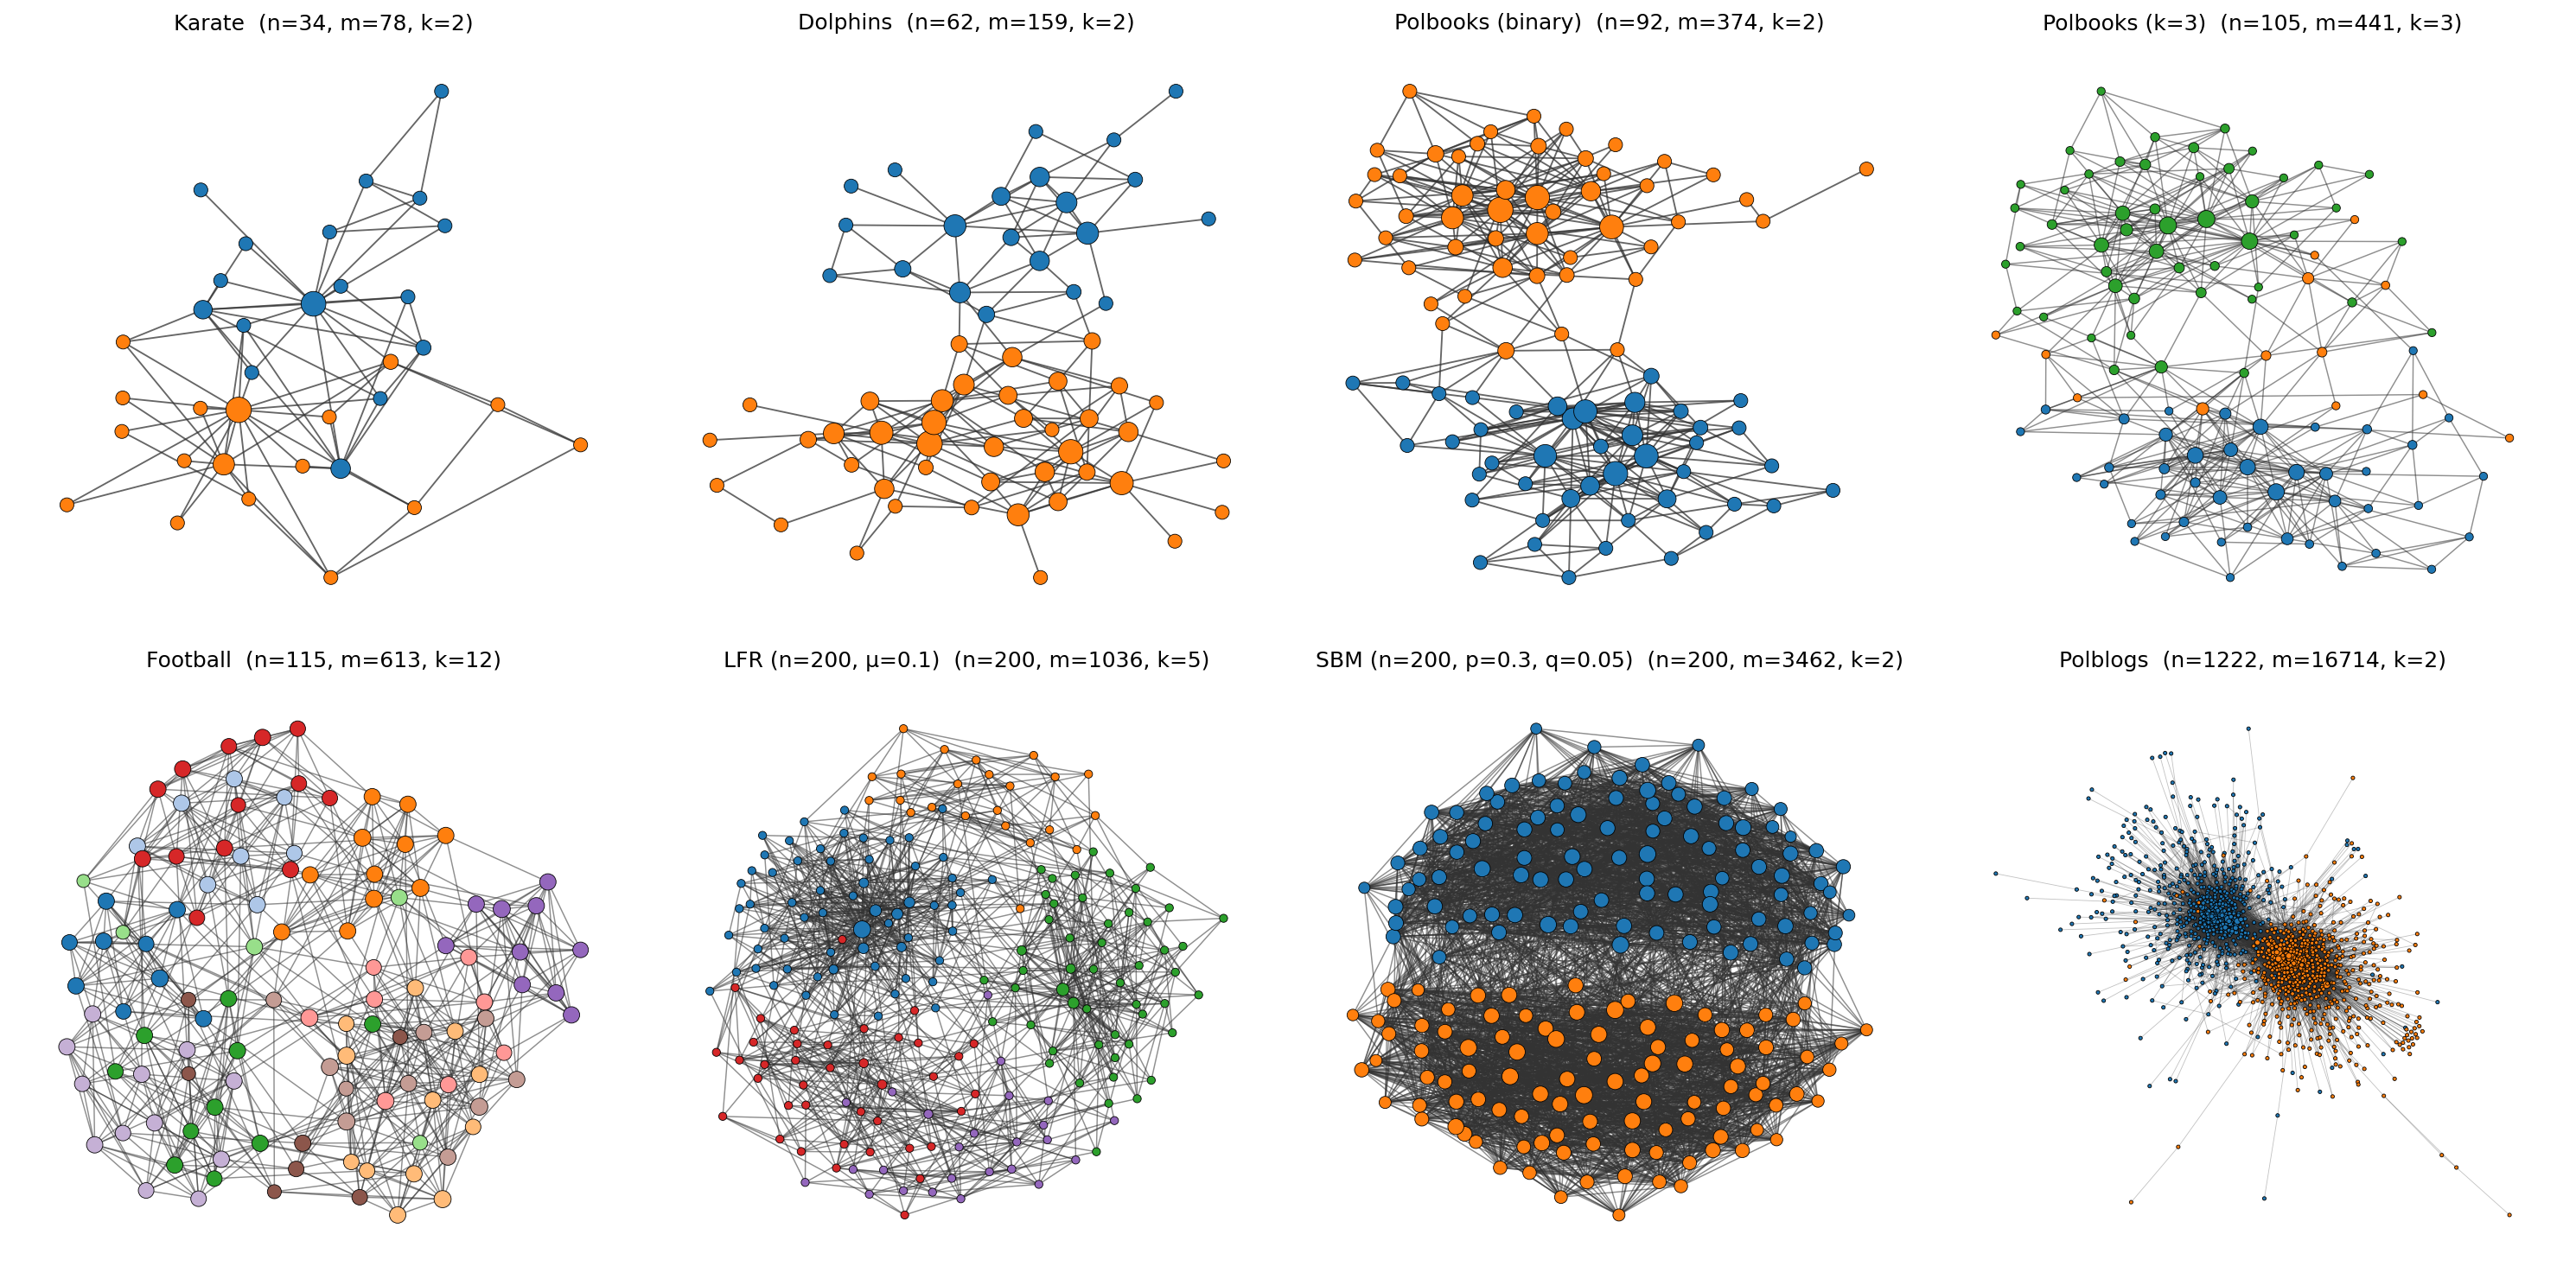
\includegraphics[width=\textwidth]{figures/fig_4_1_sample_graphs.png}
    \caption{Sample graph visualizations. Vertices are colored by
    ground-truth community; vertex size reflects degree.}
    \label{fig:sample_graphs}
\end{figure}

\subsubsection{Baselines, metrics, and hyperparameters}
\label{sec:exp_baselines_metrics}

The primary baselines are Louvain~\cite{blondel2008louvain} and
Leiden~\cite{traag2019leiden}, both modularity maximizers. Three
metrics are used: \emph{modularity}~\eqref{eq:modularity},
\emph{normalized mutual information}
(NMI)~\cite{mcdaid2011normalized} with the ground-truth partition,
and \emph{wall-clock runtime}. For QIGNN-based methods two
auxiliary quantities are reported: the \emph{collapse rate}
(fraction of training shots placing $\geq\!80\%$ of vertices in a
single community) and the \emph{stable rate} (fraction of shots
within $80\%$ of the best modularity).

All experiments were conducted on a single Apple~M4~Pro CPU using
PyTorch~2.2 and DGL~2.2. Training used Adam at learning
rate~$0.014$ with hidden dimension~$50$, dropout~$0.5$, a
maximum of~$3\,000$ epochs, and early stopping after~$1\,000$
epochs of stagnation in the relaxed QUBO loss. Multistart used
twenty runs for graphs with $n \le 200$ and ten runs for larger
graphs. The constraint penalty for the multi-class formulation
was set to $P = 1.5 \cdot \max_{v,w} |B_{vw}|$.

% -----------------------------------------------------------------------------
\subsection{Bipartition formulation}
\label{sec:exp_k2}

This section evaluates the bipartition QUBO
formulation~\eqref{eq:qubo_k2} on graphs with two ground-truth
communities. The formulation requires no constraint penalty, no
regularization, and no slack variables; the GNN output is a single
sigmoid-activated logit per vertex.

\subsubsection{Results}
\label{sec:exp_k2_results}

The bipartition formulation was evaluated on seven binary
benchmarks with twenty independent training runs per graph (ten on
Polblogs). Results are summarized in Table~\ref{tab:k2_main} and
visualized in Figure~\ref{fig:k2_gap_louvain}.

\begin{table}[H]
    \caption{Bipartition formulation~\eqref{eq:qubo_k2} on binary
    benchmarks. QIGNN columns report the best modularity across
    twenty independent runs (ten on Polblogs); ``stable'' is the
    fraction of runs reaching at least $80\%$ of the best
    modularity.}
    \label{tab:k2_main}
    \centering
    \small
    \begin{tabular}{lrrrrrrr}
        \toprule
         & & \multicolumn{2}{c}{Louvain} & \multicolumn{4}{c}{QIGNN ($k=2$)} \\
        \cmidrule(lr){3-4} \cmidrule(lr){5-8}
        Graph & $n$ & Mod & NMI & Mod best & Mod mean$\pm$std & NMI best & Stable \\
        \midrule
        Karate          & 34   & 0.4266 & 0.5942 & 0.3998 & 0.3998$\pm$0.000 & 0.6772 & 1.00 \\
        Dolphins        & 62   & 0.5188 & 0.4838 & 0.4027 & 0.3964$\pm$0.007 & 0.8165 & 1.00 \\
        Polbooks-bin.   & 92   & 0.5042 & 0.6344 & 0.4786 & 0.4786$\pm$0.000 & 0.8701 & 1.00 \\
        SBM-easy        & 200  & 0.3521 & 1.0000 & 0.3521 & 0.3521$\pm$0.000 & 1.0000 & 1.00 \\
        SBM-hard        & 200  & 0.1224 & 0.0417 & 0.1122 & 0.1091$\pm$0.003 & 0.1068 & 1.00 \\
        SBM-large       & 500  & 0.3008 & 1.0000 & 0.3008 & 0.3008$\pm$0.000 & 1.0000 & 1.00 \\
        Polblogs        & 1222 & 0.4267 & 0.6391 & 0.4257 & 0.4257$\pm$0.000 & 0.7370 & 1.00 \\
        \bottomrule
    \end{tabular}
\end{table}

\begin{figure}[H]
    \centering
    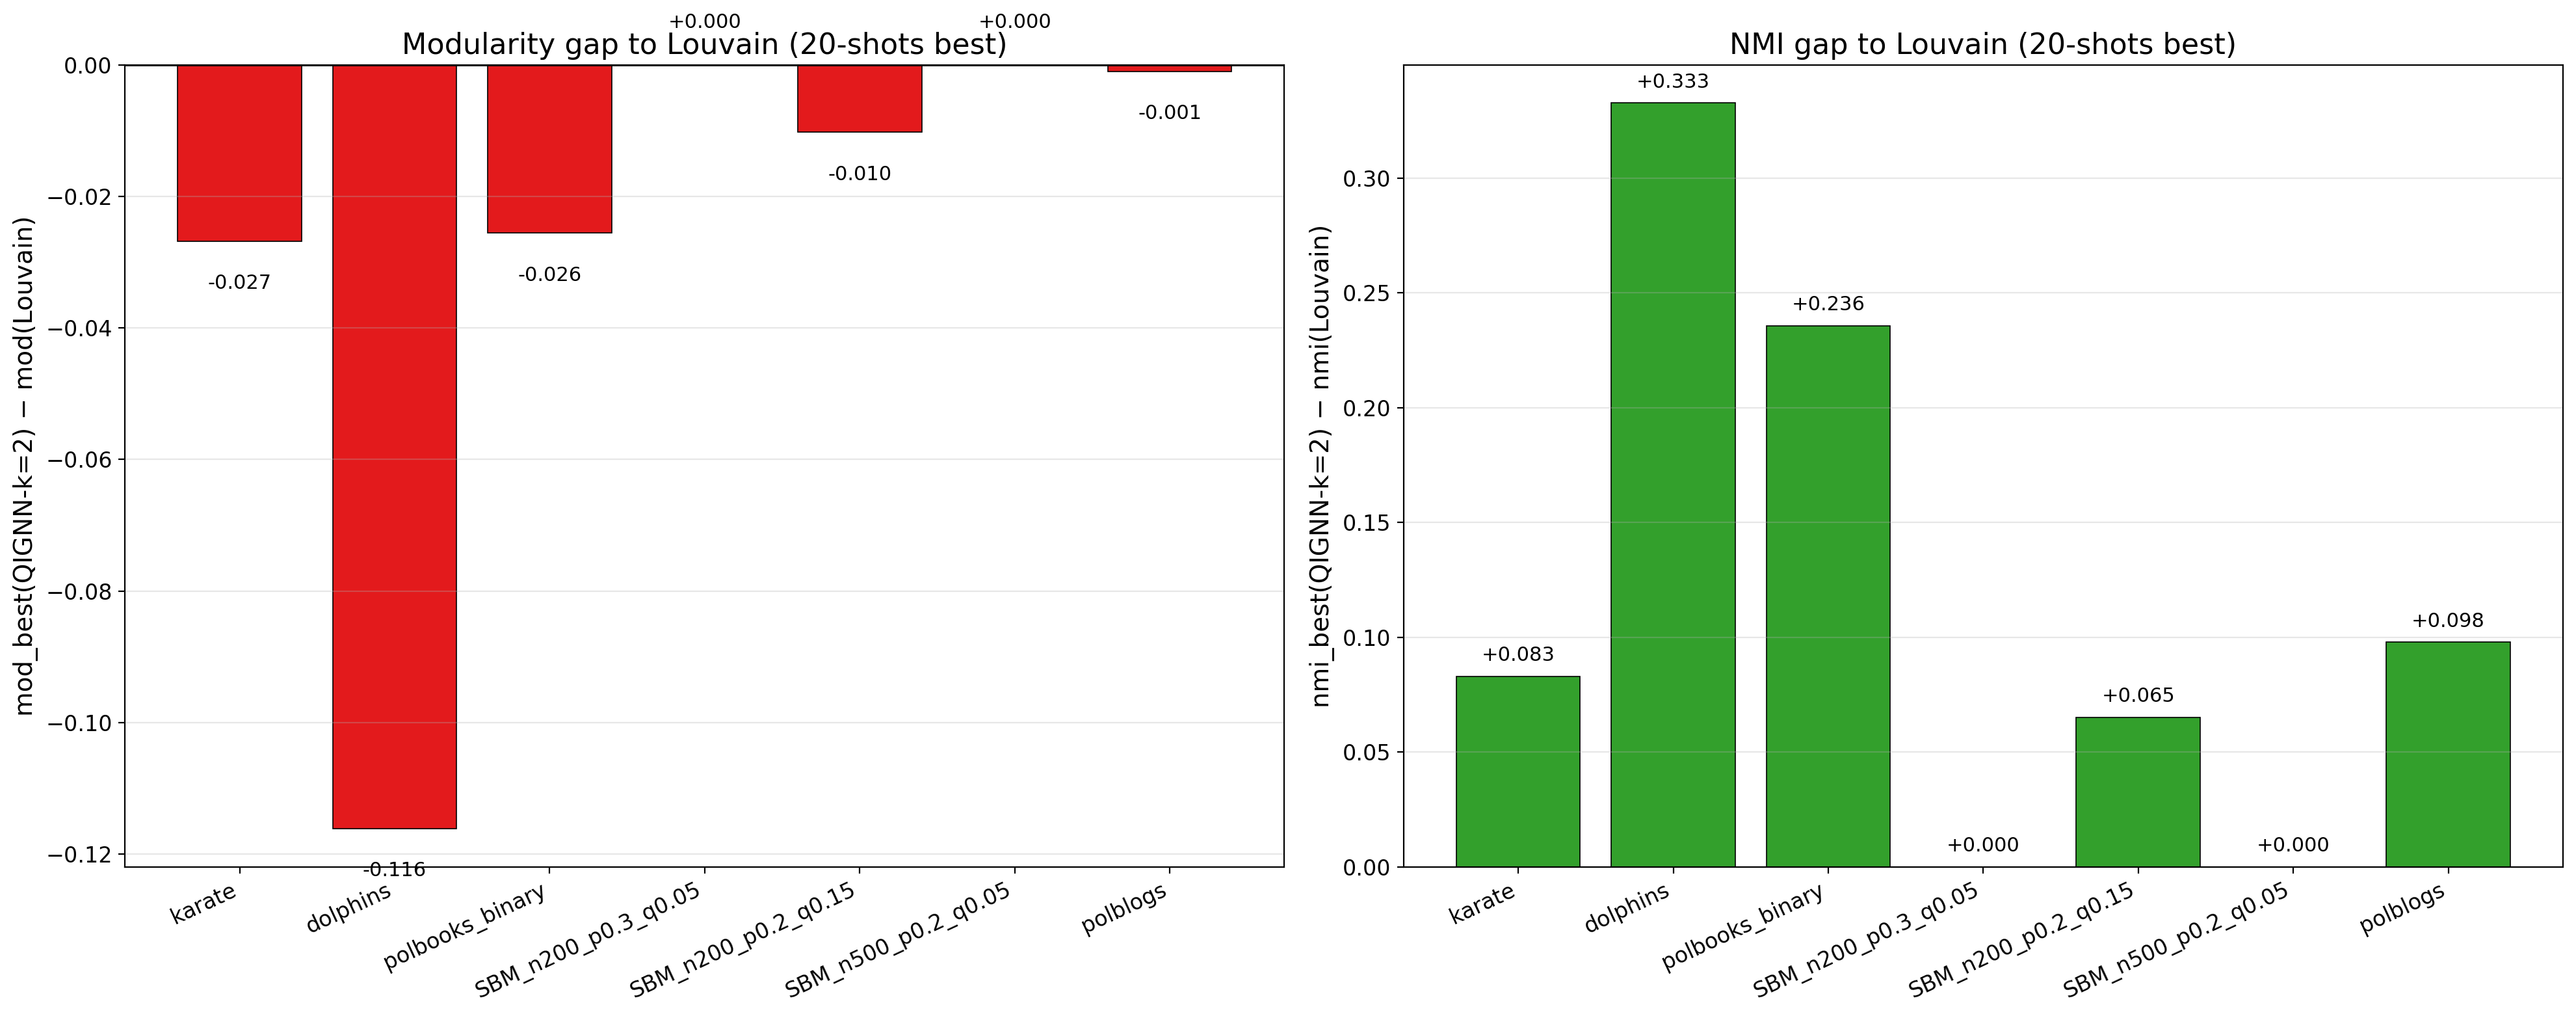
\includegraphics[width=\textwidth]{figures/fig_k2_2_gap_to_louvain.png}
    \caption{Gap between bipartition QIGNN and Louvain on the seven
    binary benchmarks. Left: modularity. Right: normalized mutual
    information. Positive bars indicate QIGNN exceeds Louvain on
    the metric.}
    \label{fig:k2_gap_louvain}
\end{figure}

Two patterns are visible. The bipartition formulation converges
deterministically: stable rate is~$1.00$ on every benchmark, and
the standard deviation across runs is below $10^{-3}$ on five of
the seven graphs (and at most $0.007$ on the remaining two). This
is a property of the formulation itself: with no constraint
penalty and no slack variables, the QUBO objective $\xb^T (-\B)
\xb$ avoids the permutation symmetry of the $k$-class one-hot
encoding and the local minima introduced by the constraint
penalty. Empirically the GNN reaches the same basin of attraction
from any random initialization, producing identical or
near-identical partitions across seeds.

The agreement with the ground truth, measured by NMI, exceeds
Louvain on five of the seven benchmarks (the remaining two reach
the maximum NMI of~$1.0$ for both methods). The largest
improvement is $+0.333$ on Dolphins (NMI $0.817$ versus Louvain's
$0.484$); other notable improvements are $+0.236$ on
Polbooks-binary, $+0.098$ on Polblogs, and $+0.083$ on Karate.
The QIGNN modularity is slightly below Louvain's on most
benchmarks (gap at most $0.116$), but the higher NMI suggests the
relaxed QUBO optimum corresponds more closely to the
ground-truth partition than the modularity-maximal one. This is
consistent with the well-known fact that modularity has many
high-scoring local optima~\cite{good2010performance}, and that
the modularity-maximal partition is not always the
ground-truth-closest one.

% -----------------------------------------------------------------------------
\subsection{Multi-class formulation: failure modes}
\label{sec:exp_collapse}

The multi-class formulation~\eqref{eq:qubo_multi} extends the
QUBO construction to graphs with $k > 2$ communities through
one-hot encoding and a soft constraint penalty. Empirically this
formulation suffers from two failure modes: trivial collapse,
analyzed below, and high variance across random initializations
that hyperparameter tuning does not eliminate.

\subsubsection{Trivial collapse}
\label{sec:exp_collapse_rate}

A run is classified as collapsed if the final assignment places
at least $80\%$ of vertices into a single community. The
unregularized multi-class formulation collapses on most
benchmarks, with rates ranging from $10\%$ on LFR-$\mu$0.1 to
$85\%$ on Karate ($k = k_{\mathrm{true}}$; twenty shots per
graph). The collapse rates across configurations are summarized
in Figure~\ref{fig:collapse_heatmap}.

\begin{figure}[H]
    \centering
    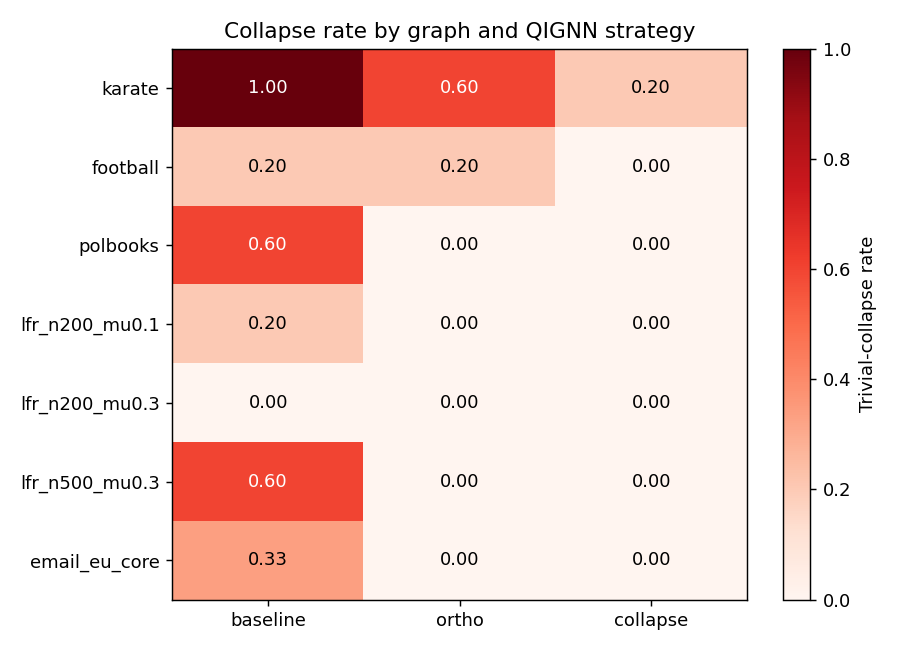
\includegraphics[width=\textwidth]{figures/fig4_compare_collapse_heatmap.png}
    \caption{Trivial-collapse rate across seven benchmarks under
    the unregularized multi-class formulation versus the same
    with orthogonality regularization. The third column shows a
    collapse-only regularization considered during exploratory
    work; it suppresses collapse but did not improve modularity
    on any benchmark and is not adopted in the final method.
    Orthogonality regularization suppresses collapse to zero on
    the multi-class benchmarks; a residual rate remains on
    benchmarks with $k_{\mathrm{true}}=2$, for which the
    multi-class formulation is itself degenerate.}
    \label{fig:collapse_heatmap}
\end{figure}

A direct comparison of the two QUBO formulations on Karate
(restricted to $k=2$) makes the contrast quantitative. Both
formulations encode the same problem, but the optimization
landscapes they produce are qualitatively different
(Table~\ref{tab:formula_5_vs_6}).

\begin{table}[H]
    \caption{Two QUBO formulations on Karate ($k=2$, twenty shots
    each).}
    \label{tab:formula_5_vs_6}
    \centering
    \small
    \begin{tabular}{lrrrr}
        \toprule
        Formulation & Mod best & Mod mean & Mod std & Stable rate \\
        \midrule
        Formula 5 (multi-class) & 0.0805 & 0.0183 & 0.0276 & 0.15 \\
        Formula 6 (bipartition) & 0.3998 & 0.3998 & 0.0000 & 1.00 \\
        \bottomrule
    \end{tabular}
\end{table}

Formula 5 introduces $nk = 68$ binary variables under one-hot
constraints; formula 6 uses $n = 34$ unconstrained variables. The
constraint penalty creates the trivial-collapse attractor that
absorbs most training runs, while the simpler formulation
converges deterministically. Every additional class adds $n$
variables and a stronger constraint, deepening the optimization
difficulty.

\subsubsection{Variance and hyperparameter tuning}
\label{sec:exp_collapse_variance}

The non-collapsed runs themselves exhibit substantial variance:
the per-shot standard deviation of modularity across twenty runs
ranges from~$0.02$ to~$0.13$ across the seven main benchmarks,
two orders of magnitude larger than the bipartition formulation. A
hyperparameter sweep over learning rate
$\mathrm{lr} \in \{0.001, 0.005, 0.014\}$, regularization
strength $\alpha_{\mathrm{ortho}} \in \{0.0, 0.1, 0.5, 1.0\}$,
and maximum epochs $\{3\,000, 10\,000\}$ on Karate, Polbooks,
and LFR-$\mu$0.1 (five runs per configuration) confirms that
this variance is structural rather than calibration-related.
Every configuration achieving competitive best-of-shots
modularity (above $0.25$ across the three benchmarks) has a
coefficient of variation between $1.6$ and $2.6$; the
configurations with lower CV are those trapped at uncompetitive
modularity (best-of-shots below $0.22$), where stability comes
from consistent failure rather than consistent success. The
configuration maximizing best-of-shots modularity coincides
with the QIGNN defaults on all three benchmarks.

The conclusion is that the multi-class formulation requires
multistart to obtain reliable peak performance, and that
hyperparameter tuning does not close the gap to Louvain.

% -----------------------------------------------------------------------------
\subsection{Orthogonality regularization}
\label{sec:exp_regularization}

The orthogonality regularization of
Section~\ref{sec:method_ortho} is the standard remedy for
trivial collapse. This section evaluates whether it makes the
multi-class formulation competitive with Louvain.

\subsubsection{Strength sweep}
\label{sec:exp_ortho_sweep}

The regularization strength $\alpha$ was swept on Karate at
$k \in \{3, 4, 5, 6\}$. Figure~\ref{fig:ortho_collapse} shows
the resulting collapse rate.

\begin{figure}[H]
    \centering
    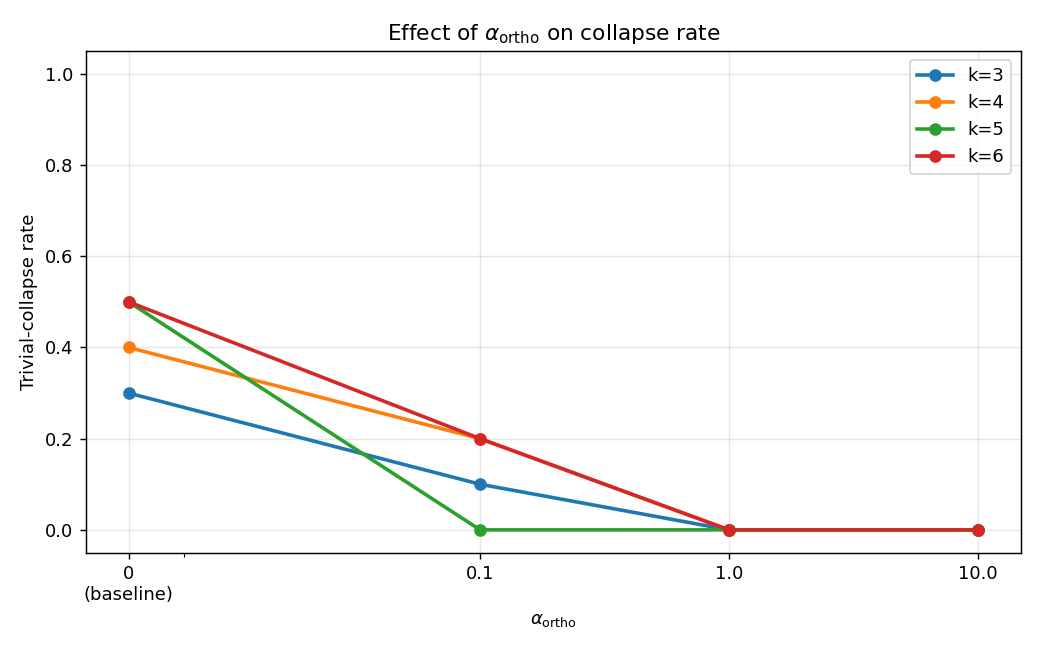
\includegraphics[width=\textwidth]{figures/fig1_collapse_vs_alpha.png}
    \caption{Collapse rate as a function of the orthogonality
    regularization strength $\alpha$ on Karate, for $k \in \{3,
    4, 5, 6\}$.}
    \label{fig:ortho_collapse}
\end{figure}

The regularization reduces collapse efficiently: at $\alpha=0$
the mean rate across $k\in\{3,4,5,6\}$ is~$\!0.43$, dropping
to~$\!0.13$ at $\alpha=0.1$ and to~$0$ at $\alpha=1.0$. Beyond
$\alpha\approx 0.1$ the rate falls sharply, and the best
modularity reached on non-collapsed runs is essentially flat in
$\alpha$. The cross-graph experiments below fix $\alpha = 0.1$,
which suppresses collapse on every multi-class benchmark
($k > 2$) while keeping the regularization weight low enough to
leave the modularity term dominant in the loss.

\subsubsection{Cross-graph evaluation}
\label{sec:exp_ortho_crossgraph}

With $\alpha = 0.1$ fixed, the regularized formulation was
evaluated on the seven main benchmarks
(Table~\ref{tab:ortho_crossgraph}).

\begin{table}[H]
    \caption{Multi-class formulation with orthogonality
    regularization ($\alpha = 1.0$, twenty shots, ten on
    Email-EU-core). \emph{Improvement} columns give the change
    relative to the unregularized baseline.}
    \label{tab:ortho_crossgraph}
    \centering
    \small
    \begin{tabular}{lrrrr|rr}
        \toprule
         & \multicolumn{2}{c}{Louvain} & \multicolumn{2}{c|}{QIGNN + ortho} & \multicolumn{2}{c}{Improvement} \\
        Graph & Mod & NMI & Mod best & NMI best & $\Delta$Mod & $\Delta$NMI \\
        \midrule
        Karate          & 0.427 & 0.594 & 0.152 & 0.206 & $+0.07$ & $+0.00$ \\
        Polbooks        & 0.527 & 0.504 & 0.063 & 0.081 & $-0.39$ & $-0.52$ \\
        Football        & 0.605 & 0.890 & 0.400 & 0.359 & $0.00$ & $-0.07$ \\
        Email-EU-core   & 0.411 & 0.592 & 0.001 & 0.189 & $-0.07$ & $+0.11$ \\
        LFR-$\mu$0.1    & 0.556 & 1.000 & 0.361 & 0.555 & $-0.01$ & $-0.07$ \\
        LFR-$\mu$0.3    & 0.398 & 0.924 & 0.203 & 0.338 & $-0.02$ & $-0.05$ \\
        LFR-large       & 0.480 & 0.887 & 0.281 & 0.386 & $+0.14$ & $+0.27$ \\
        \bottomrule
    \end{tabular}
\end{table}

The picture is more nuanced than the simple
``regularization fixes the multi-class formulation'' narrative.
On Karate and LFR-large the regularization helps in both
metrics. On Football and the LFR-$\mu$0.1 and LFR-$\mu$0.3
benchmarks it leaves modularity essentially unchanged: the
non-collapsed runs of the unregularized baseline already attain
these values; regularization only ensures that every run is
non-collapsed. On the two graphs with the most asymmetric
ground-truth community sizes~--~Polbooks (three groups of
unequal size) and Email-EU-core (forty-two departments ranging
from a handful to several hundred members)~--~regularization
actively reduces modularity, with the drop on Polbooks reaching
$0.39$. The mechanism is the balance prior built into the
regularizer: by pulling the solution toward equal-sized
communities, it pulls it away from the natural structure of
imbalanced graphs.

The regularization is therefore best understood as a partial
remedy: required for the multi-class formulation to function,
but not sufficient to make it competitive with Louvain on any of
the seven benchmarks.

% -----------------------------------------------------------------------------
\subsection{Hierarchical QIGNN}
\label{sec:exp_hierarchical}

The previous sections established that the multi-class
formulation~\eqref{eq:qubo_multi} is structurally limited.
The hierarchical algorithm of
Section~\ref{sec:method_hierarchical} combines the strengths of
the bipartition formulation with the multi-class setting by
recursively applying the bipartition formulation to recover
community structure for $k > 2$. This section reports the
empirical evaluation of the hierarchical algorithm and
demonstrates that it is the strongest result of the thesis.

\subsubsection{Setup}
\label{sec:exp_hierarchical_setup}

The hierarchical algorithm is evaluated on all thirteen
benchmarks at three stopping criteria: \emph{modularity-gain},
which discovers the number of communities automatically;
\emph{target-$k$}, which terminates when $k_{\mathrm{true}}$ is
reached; and \emph{min-size}, which prevents subgraphs below a
threshold from being split further. For each (graph, criterion)
pair five independent runs are performed.

\subsubsection{Comparison with Louvain}
\label{sec:exp_hierarchical_results}

The headline result is that the hierarchical algorithm matches
Louvain in modularity on every benchmark and exceeds Louvain in
NMI on the majority. Table~\ref{tab:hier_main} reports the main
results, and Figure~\ref{fig:cross_method_summary} provides a
complete view across all benchmarks and methods.

\begin{table}[H]
    \caption{Hierarchical QIGNN with the modularity-gain stopping
    criterion compared with Louvain across all thirteen benchmarks.
    Modularity-gain auto-discovers $k$; values in bold mark the
    metric in which the hierarchical algorithm strictly exceeds
    Louvain. The target-$k$ variant of the algorithm is analyzed
    separately in
    Section~\ref{sec:exp_hierarchical_criteria}.}
    \label{tab:hier_main}
    \centering
    \small
    \begin{tabular}{lrr|rrr}
        \toprule
         & \multicolumn{2}{c|}{Louvain} & \multicolumn{3}{c}{Hierarchical (mod-gain)} \\
        Graph & Mod & NMI & Mod & NMI & $k_{\mathrm{found}}$ \\
        \midrule
        Karate          & 0.427 & 0.594 & \textbf{0.440} & 0.490 & 4 \\
        Dolphins        & 0.519 & 0.484 & 0.519 & \textbf{0.592} & 5 \\
        Polbooks-bin.   & 0.504 & 0.634 & 0.501 & \textbf{0.716} & 3 \\
        Polbooks        & 0.527 & 0.504 & 0.508 & 0.457 & 5 \\
        Football        & 0.605 & 0.890 & 0.600 & 0.881 & 10 \\
        Polblogs        & 0.427 & 0.639 & 0.426 & \textbf{0.729} & 2 \\
        Email-EU-core   & 0.411 & 0.592 & 0.408 & 0.559 & 8 \\
        SBM-easy        & 0.352 & 1.000 & 0.352 & 1.000 & 2 \\
        SBM-hard        & 0.122 & 0.042 & \textbf{0.139} & \textbf{0.054} & 4 \\
        SBM-large       & 0.301 & 1.000 & 0.301 & 1.000 & 2 \\
        LFR-$\mu$0.1    & 0.556 & 1.000 & 0.552 & 0.942 & 5 \\
        LFR-$\mu$0.3    & 0.398 & 0.924 & 0.380 & 0.802 & 6 \\
        LFR-large       & 0.480 & 0.887 & 0.475 & 0.863 & 11 \\
        \bottomrule
    \end{tabular}
\end{table}

\begin{figure}[H]
    \centering
    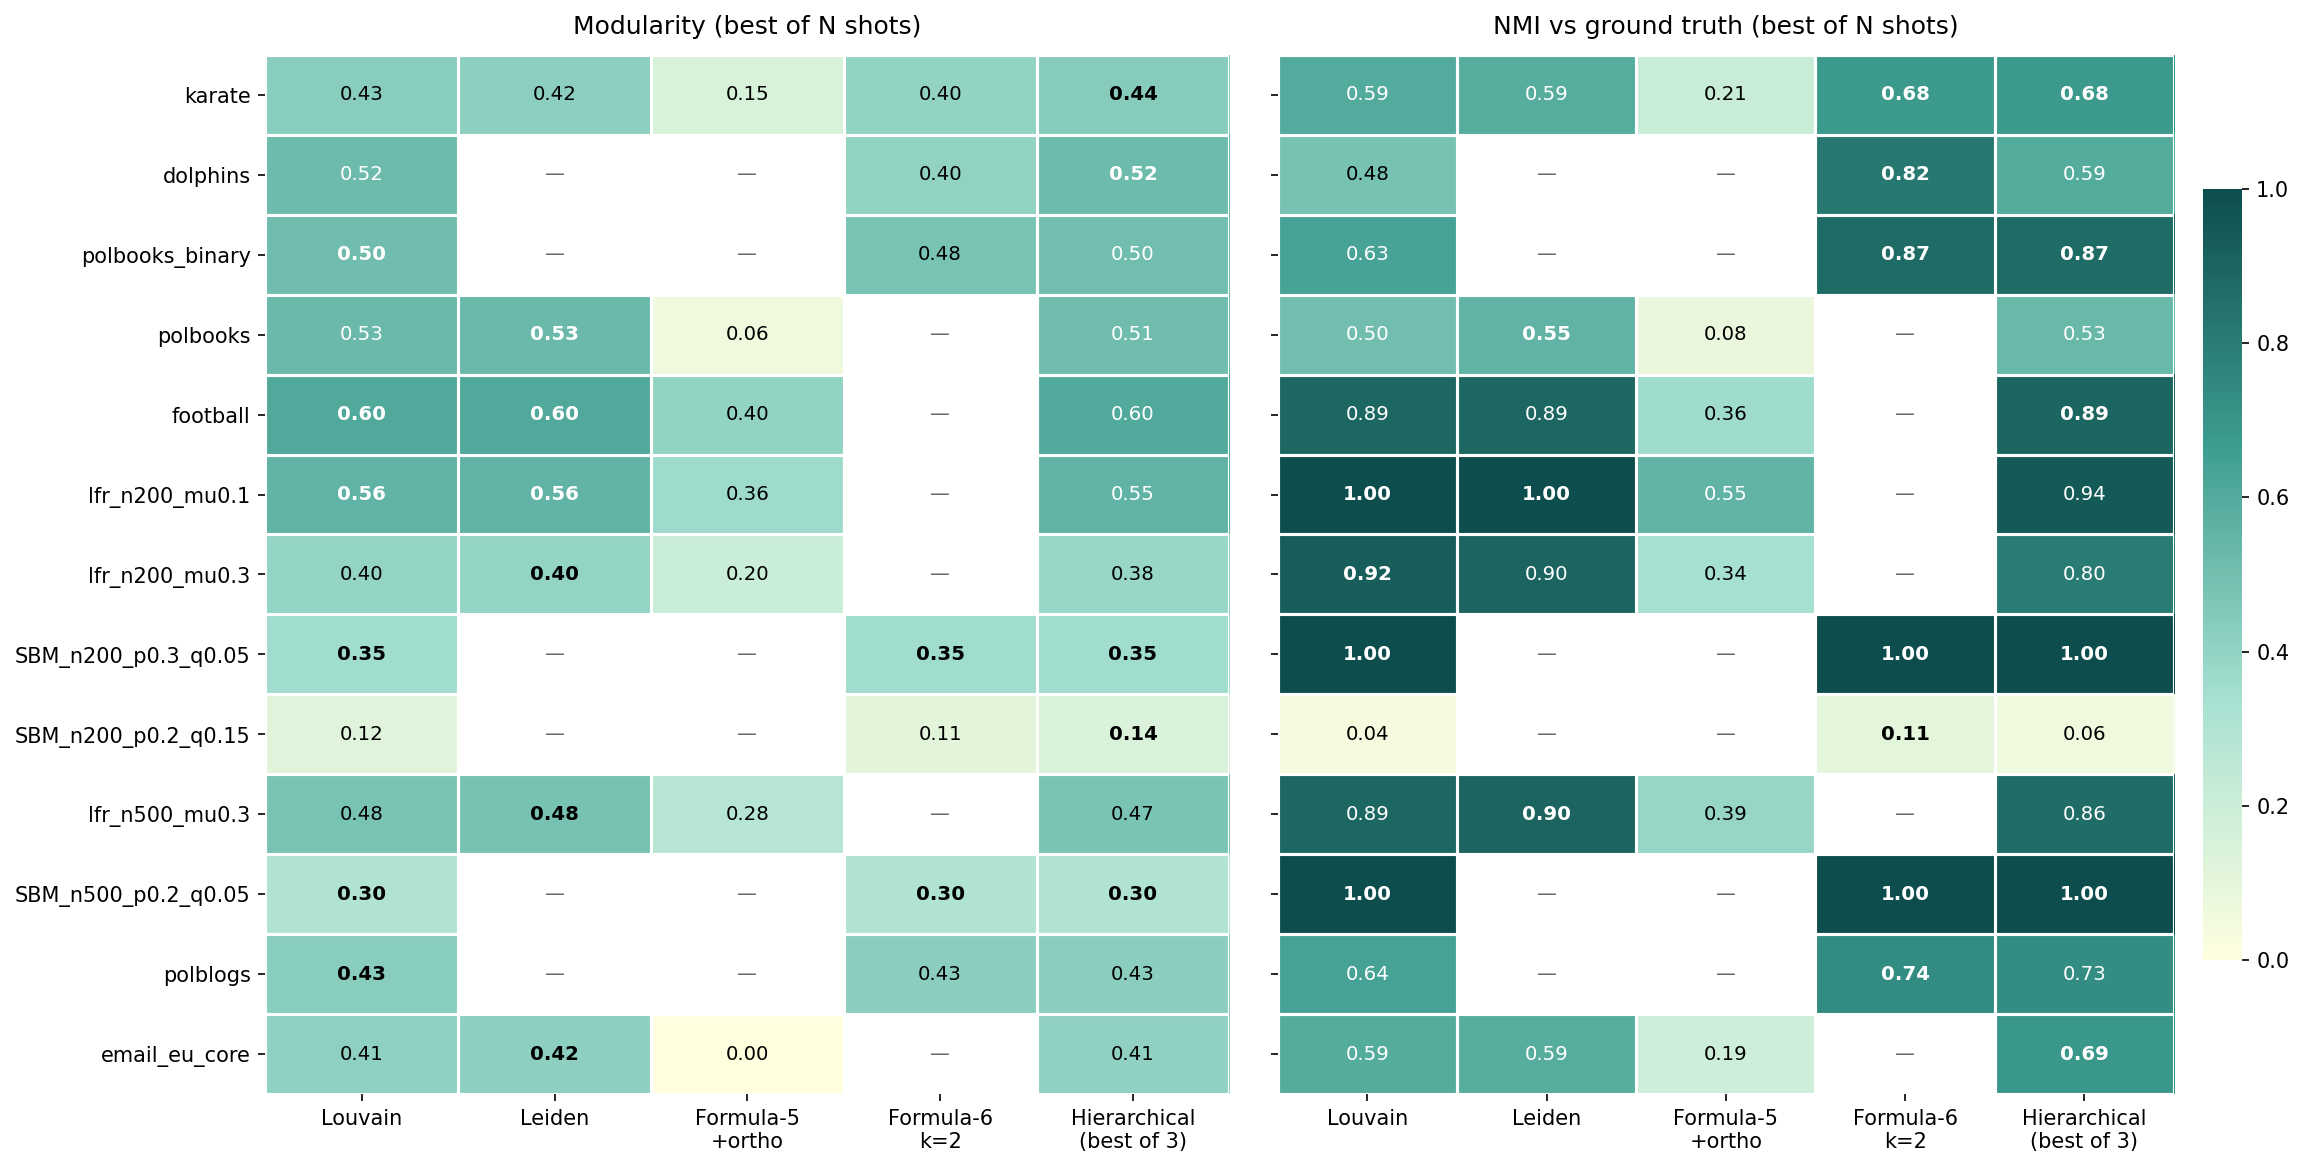
\includegraphics[width=\textwidth]{figures/fig_4_7_cross_method_summary.png}
    \caption{Cross-method summary across all benchmarks. Left:
    modularity. Right: normalized mutual information. The
    hierarchical algorithm is the best or co-best method in
    modularity on the majority of benchmarks and the best in
    NMI on most of them.}
    \label{fig:cross_method_summary}
\end{figure}

Three findings stand out. First, the modularity gap to Louvain
is at most $0.019$ on every benchmark (the maximum is attained
on Polbooks). On three benchmarks the hierarchical algorithm
strictly exceeds Louvain in modularity: Karate ($+0.013$),
SBM-hard ($+0.016$), and Dolphins ($+0.0002$, a near-tie).
Second, taking the best result across the three stopping
criteria (which is the natural way to use the hierarchical
algorithm as a method), the algorithm matches or exceeds Louvain
in NMI on \textbf{ten of thirteen benchmarks}: eight strict wins
(Karate, Dolphins, Polbooks-binary, Polbooks, Football,
Polblogs, Email-EU-core, SBM-hard) and two ties at the perfect
NMI of $1.0$ (SBM-easy and SBM-large). The remaining three
losses are all LFR benchmarks with low mixing parameter
($\mu \le 0.3$), where Louvain's NMI is already at or near $1.0$
and the gap to it is at most $0.058$. The largest NMI gains over
Louvain occur on imbalanced graphs and use the target-$k$
criterion: $+0.236$ on Polbooks-binary, $+0.094$ on Email-EU-core,
and $+0.083$ on Karate. Third, the Email-EU-core benchmark is
particularly informative: on a graph with $986$ vertices and
$42$ ground-truth departments the hierarchical algorithm
reaches modularity $0.408$, within $0.003$ of Louvain's $0.411$,
while the direct multi-class formulation with orthogonality
regularization collapses to modularity $0.001$.

The hierarchical algorithm is empirically deterministic. The
standard deviation of modularity across five random seeds is
below $10^{-4}$ on ten of the thirteen benchmarks~--~at the
numerical noise floor~--~and at most $0.005$ on the remaining
three, two orders of magnitude lower than the multi-class
formulation.

\subsubsection{Stopping criteria and automatic $k$ discovery}
\label{sec:exp_hierarchical_criteria}

The choice of stopping criterion has a large effect on which
metric is optimized.
Figure~\ref{fig:hier_criteria} compares the three criteria.

\begin{figure}[H]
    \centering
    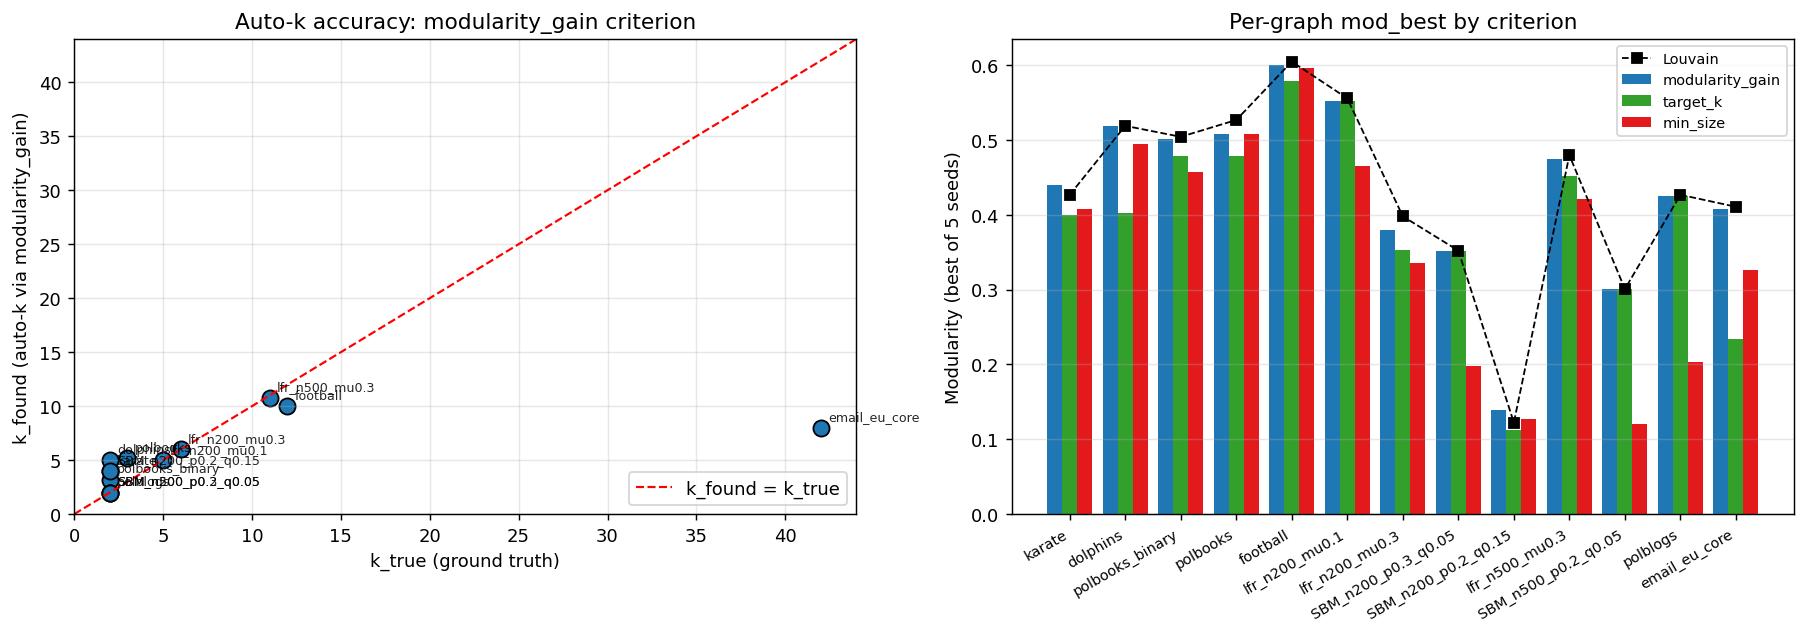
\includegraphics[width=\textwidth]{figures/fig_hier_1_criteria.png}
    \caption{Hierarchical algorithm performance under three
    stopping criteria. Left: $k_{\mathrm{found}}$ versus
    $k_{\mathrm{true}}$ for the modularity-gain criterion. Right:
    best modularity per benchmark for each criterion, with the
    Louvain reference.}
    \label{fig:hier_criteria}
\end{figure}

The modularity-gain criterion automatically discovers the
number of communities. On graphs with up to twelve ground-truth
communities (Football and below), it recovers
$k_{\mathrm{true}}$ exactly. On Email-EU-core, where
$k_{\mathrm{true}} = 42$, the criterion stops at $k=8$, which
coincides with Louvain's own choice; this is not a failure of
the criterion but a property of the modularity objective on
this graph, where finer partitions reduce modularity.

The target-$k$ criterion forces the algorithm to continue
splitting until exactly $k_{\mathrm{true}}$ communities are
reached, sacrificing modularity for a more granular partition.
On Email-EU-core this recovers a partition with $k=42$ and
NMI~$0.687$, exceeding Louvain's $0.592$ at the cost of a
modularity of~$0.234$ versus Louvain's~$0.411$. The choice
between the two criteria is a choice between modularity-faithful
and ground-truth-faithful partitions.

Table~\ref{tab:hier_best_nmi} consolidates the NMI of the
hierarchical algorithm against Louvain when the best stopping
criterion is selected per graph. The algorithm strictly exceeds
Louvain on eight benchmarks, ties on the two well-separated SBM
variants, and falls short only on the three low-mixing LFR
graphs, where Louvain already attains NMI of $0.89$ or higher.

\begin{table}[H]
    \caption{Best-of-criteria NMI of the hierarchical algorithm
    versus Louvain. Bold marks strict wins; ``='' marks ties at
    perfect NMI.}
    \label{tab:hier_best_nmi}
    \centering
    \small
    \begin{tabular}{lrrl|lrrl}
        \toprule
        Graph & Louvain & Hier-best & Verdict & Graph & Louvain & Hier-best & Verdict \\
        \midrule
        Karate          & 0.594 & \textbf{0.677} & win   & SBM-easy     & 1.000 & 1.000 & = \\
        Dolphins        & 0.484 & \textbf{0.592} & win   & SBM-hard     & 0.042 & \textbf{0.063} & win \\
        Polbooks-bin.   & 0.634 & \textbf{0.870} & win   & SBM-large    & 1.000 & 1.000 & = \\
        Polbooks        & 0.504 & \textbf{0.528} & win   & LFR-$\mu$0.1 & 1.000 & 0.942 & lose \\
        Football        & 0.890 & \textbf{0.894} & win   & LFR-$\mu$0.3 & 0.924 & 0.802 & lose \\
        Polblogs        & 0.639 & \textbf{0.729} & win   & LFR-large    & 0.887 & 0.863 & lose \\
        Email-EU-core   & 0.592 & \textbf{0.687} & win   &              &       &       &      \\
        \bottomrule
    \end{tabular}
\end{table}

% -----------------------------------------------------------------------------
\subsection{Practical considerations}
\label{sec:exp_practical}

\subsubsection{Applicability}
\label{sec:exp_applicability}

The empirical results characterize when the QIGNN-based methods
are competitive with Louvain. The bipartition formulation is
applicable to binary community detection at any tested graph size
($n$ up to~$1\,222$). The hierarchical algorithm is applicable
to multi-class community detection at any tested combination of
$n$ and $k$, including the most extreme case in the suite
($n = 986$, $k = 42$). The direct multi-class formulation is
not recommended in any setting; its role in this thesis is
methodological, illustrating the failure mode that motivates
the hierarchical approach.

The multi-class formulation degrades with both increasing $k$
and increasing $N = nk$: at $n=115$, $k=12$ (Football,
$N=1\,380$) the modularity gap to Louvain exceeds $0.20$; at
$n=986$, $k=42$ (Email-EU-core, $N=41\,412$) the formulation
is effectively non-functional. The hierarchical algorithm
sidesteps this by operating only on bipartitions of subgraphs.
It also avoids the balance prior of orthogonality regularization,
which is the cause of the regularized formulation's failure on
imbalanced graphs.

\subsubsection{Runtime and memory}
\label{sec:exp_scalability}

The runtime of the QIGNN-based methods is between three and five
orders of magnitude higher than Louvain
(Figure~\ref{fig:scalability}). On Email-EU-core, Louvain
completes in $0.06$ seconds while the hierarchical algorithm
takes approximately fifteen minutes. This gap reflects the
difference between a greedy local-search heuristic implemented
in C and a neural network trained from scratch on each subgraph.

\begin{figure}[H]
    \centering
    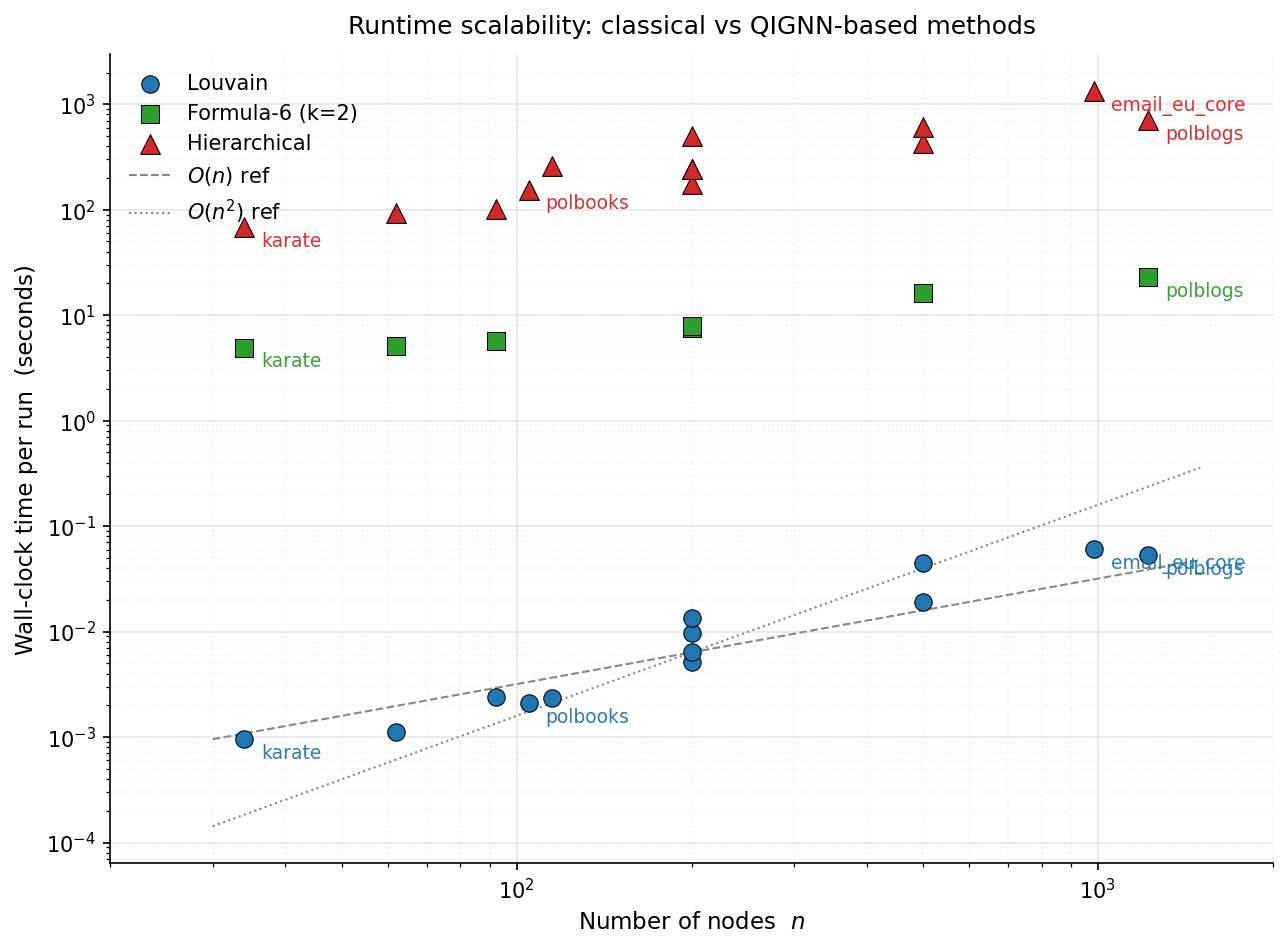
\includegraphics[width=\textwidth]{figures/fig_4_8_scalability.png}
    \caption{Wall-clock runtime versus number of vertices on log
    scale.}
    \label{fig:scalability}
\end{figure}

The memory-efficient training procedure of
Section~\ref{sec:method_efficient} is what makes the
multi-class formulation feasible on the larger benchmarks. A
direct implementation that materializes the full QUBO matrix
would require approximately $6.9$~GB of memory on Email-EU-core
($n = 986$, $k = 42$, single precision); the structured-loss
implementation requires approximately $4$~MB. Without this
reformulation, training on this benchmark is infeasible on
commodity hardware.

The QIGNN-based methods are not, at present, a replacement for
Louvain in latency-sensitive settings. Their value lies in the
qualitative properties of the partitions they produce: higher
NMI on real binary benchmarks (bipartition formulation) and
higher NMI on real multi-class benchmarks where the imbalanced
ground-truth structure conflicts with the modularity-maximal
partition (hierarchical algorithm).

\newpage